%%%%%%%%%%%%%%%%%%%%%%%%%%%%%%%%%%%%%%%%%
% Lachaise Assignment
% LaTeX Template
% Version 1.0 (26/6/2018)
%
% This template originates from:
% http://www.LaTeXTemplates.com
%
% Authors:
% Marion Lachaise & François Févotte
% Vel (vel@LaTeXTemplates.com)
%
% License:
% CC BY-NC-SA 3.0 (http://creativecommons.org/licenses/by-nc-sa/3.0/)
% 
%%%%%%%%%%%%%%%%%%%%%%%%%%%%%%%%%%%%%%%%%

%----------------------------------------------------------------------------------------
%	PACKAGES AND OTHER DOCUMENT CONFIGURATIONS
%----------------------------------------------------------------------------------------

\documentclass{article}

%%%%%%%%%%%%%%%%%%%%%%%%%%%%%%%%%%%%%%%%%
% Lachaise Assignment
% Structure Specification File
% Version 1.0 (26/6/2018)
%
% This template originates from:
% http://www.LaTeXTemplates.com
%
% Authors:
% Marion Lachaise & François Févotte
% Vel (vel@LaTeXTemplates.com)
%
% License:
% CC BY-NC-SA 3.0 (http://creativecommons.org/licenses/by-nc-sa/3.0/)
% 
%%%%%%%%%%%%%%%%%%%%%%%%%%%%%%%%%%%%%%%%%

%----------------------------------------------------------------------------------------
%	PACKAGES AND OTHER DOCUMENT CONFIGURATIONS
%----------------------------------------------------------------------------------------

\usepackage{amsmath,amsfonts,amssymb} % Math packages

\usepackage{enumerate} % Custom item numbers for enumerations

\usepackage[ruled]{algorithm2e} % Algorithms

\usepackage[framemethod=tikz]{mdframed} % Allows defining custom boxed/framed environments


\usepackage{listings} % File listings, with syntax highlighting
\usepackage{xcolor} % for setting colors

% set the default code style
\lstset{
	basicstyle=\ttfamily ,
    frame=tb, % draw a frame at the top and bottom of the code block
    tabsize=4, % tab space width
    showstringspaces=false, % don't mark spaces in strings
    numbers=left, % display line numbers on the left
    commentstyle=\color{gray}, % comment color
    keywordstyle=\color{blue}, % keyword color
    stringstyle=\color{magenta} % string color
}

%----------------------------------------------------------------------------------------
%	DOCUMENT MARGINS
%----------------------------------------------------------------------------------------

\usepackage{geometry} % Required for adjusting page dimensions and margins

\geometry{
	paper=a4paper, % Paper size, change to letterpaper for US letter size
	top=2.5cm, % Top margin
	bottom=3cm, % Bottom margin
	left=2.5cm, % Left margin
	right=2.5cm, % Right margin
	headheight=14pt, % Header height
	footskip=1.5cm, % Space from the bottom margin to the baseline of the footer
	headsep=1.2cm, % Space from the top margin to the baseline of the header
	%showframe, % Uncomment to show how the type block is set on the page
}

%----------------------------------------------------------------------------------------
%	FONTS
%----------------------------------------------------------------------------------------

\usepackage[utf8]{inputenc} % Required for inputting international characters
\usepackage[T1]{fontenc} % Output font encoding for international characters

%\usepackage{XCharter} % Use the XCharter fonts

%----------------------------------------------------------------------------------------
%	COMMAND LINE ENVIRONMENT
%----------------------------------------------------------------------------------------

% Usage:
% \begin{commandline}
%	\begin{verbatim}
%		$ ls
%		
%		Applications	Desktop	...
%	\end{verbatim}
% \end{commandline}

\mdfdefinestyle{commandline}{
	leftmargin=10pt,
	rightmargin=10pt,
	innerleftmargin=15pt,
	middlelinecolor=black!50!white,
	middlelinewidth=2pt,
	frametitlerule=false,
	backgroundcolor=black!5!white,
	frametitle={Command Line},
	frametitlefont={\normalfont\sffamily\color{white}\hspace{-1em}},
	frametitlebackgroundcolor=black!50!white,
	nobreak,
}

% Define a custom environment for command-line snapshots
\newenvironment{commandline}{
	\medskip
	\begin{mdframed}[style=commandline]
}{
	\end{mdframed}
	\medskip
}

%----------------------------------------------------------------------------------------
%	FILE CONTENTS ENVIRONMENT
%----------------------------------------------------------------------------------------

% Usage:
% \begin{file}[optional filename, defaults to "File"]
%	File contents, for example, with a listings environment
% \end{file}

\mdfdefinestyle{file}{
	innertopmargin=1.6\baselineskip,
	innerbottommargin=0.8\baselineskip,
	topline=false, bottomline=false,
	leftline=false, rightline=false,
	leftmargin=2cm,
	rightmargin=2cm,
	singleextra={%
		\draw[fill=black!10!white](P)++(0,-1.2em)rectangle(P-|O);
		\node[anchor=north west]
		at(P-|O){\ttfamily\mdfilename};
		%
		\def\l{3em}
		\draw(O-|P)++(-\l,0)--++(\l,\l)--(P)--(P-|O)--(O)--cycle;
		\draw(O-|P)++(-\l,0)--++(0,\l)--++(\l,0);
	},
	nobreak,
}

% Define a custom environment for file contents
\newenvironment{file}[1][File]{ % Set the default filename to "File"
	\medskip
	\newcommand{\mdfilename}{#1}
	\begin{mdframed}[style=file]
}{
	\end{mdframed}
	\medskip
}

%----------------------------------------------------------------------------------------
%	NUMBERED QUESTIONS ENVIRONMENT
%----------------------------------------------------------------------------------------

% Usage:
% \begin{question}[optional title]
%	Question contents
% \end{question}

\mdfdefinestyle{question}{
	innertopmargin=1.2\baselineskip,
	innerbottommargin=0.8\baselineskip,
	roundcorner=5pt,
	nobreak,
	singleextra={%
		\draw(P-|O)node[xshift=1em,anchor=west,fill=white,draw,rounded corners=5pt]{%
		Question \theQuestion\questionTitle};
	},
}

\newcounter{Question} % Stores the current question number that gets iterated with each new question

% Define a custom environment for numbered questions
\newenvironment{question}[1][\unskip]{
	\bigskip
	\stepcounter{Question}
	\newcommand{\questionTitle}{~#1}
	\begin{mdframed}[style=question]
}{
	\end{mdframed}
	\medskip
}

%----------------------------------------------------------------------------------------
%	WARNING TEXT ENVIRONMENT
%----------------------------------------------------------------------------------------

% Usage:
% \begin{warn}[optional title, defaults to "Warning:"]
%	Contents
% \end{warn}

\mdfdefinestyle{warning}{
	topline=false, bottomline=false,
	leftline=false, rightline=false,
	nobreak,
	singleextra={%
		\draw(P-|O)++(-0.5em,0)node(tmp1){};
		\draw(P-|O)++(0.5em,0)node(tmp2){};
		\fill[black,rotate around={45:(P-|O)}](tmp1)rectangle(tmp2);
		\node at(P-|O){\color{white}\scriptsize\bf !};
		\draw[very thick](P-|O)++(0,-1em)--(O);%--(O-|P);
	}
}

% Define a custom environment for warning text
\newenvironment{warn}[1][Warning:]{ % Set the default warning to "Warning:"
	\medskip
	\begin{mdframed}[style=warning]
		\noindent{\textbf{#1}}
}{
	\end{mdframed}
}

%----------------------------------------------------------------------------------------
%	INFORMATION ENVIRONMENT
%----------------------------------------------------------------------------------------

% Usage:
% \begin{info}[optional title, defaults to "Info:"]
% 	contents
% 	\end{info}

\mdfdefinestyle{info}{%
	topline=false, bottomline=false,
	leftline=false, rightline=false,
	nobreak,
	singleextra={%
		\fill[black](P-|O)circle[radius=0.4em];
		\node at(P-|O){\color{white}\scriptsize\bf i};
		\draw[very thick](P-|O)++(0,-0.8em)--(O);%--(O-|P);
	}
}

% Define a custom environment for information
\newenvironment{info}[1][Info:]{ % Set the default title to "Info:"
	\medskip
	\begin{mdframed}[style=info]
		\noindent{\textbf{#1}}
}{
	\end{mdframed}
}
 % Include the file specifying the document structure and custom commands

%----------------------------------------------------------------------------------------
%	ASSIGNMENT INFORMATION
%----------------------------------------------------------------------------------------

\title{C++ Programming: Think Before You Code} % Title of the assignment

\author{Nthikeng Letsoalo} % Author name and email address

\date{University of the Witwatersrand --- \today} % University, school and/or department name(s) and a date

%----------------------------------------------------------------------------------------

\begin{document}

\maketitle % Print the title

%----------------------------------------------------------------------------------------
%	INTRODUCTION
%----------------------------------------------------------------------------------------

\section*{Introduction} % Unnumbered section

Today's lab will focus primarily on your problem solving skills. The idea is to get you thinking about a problem before you actually start to write code. After having solved the problem using pen and paper (it is highly recommended that you do this), it is time to translate your thoughts into code. When solving your problem remember to use key words like \textbf{if}, \textbf{for}, \textbf{while} etc. during your thought process, this will guide your intuition when translating your thoughts to code which is the main objective. 
\\\\
For today's lab I will not be giving you any skeleton code. With that being said, I expect you to create your own functions with whatever parameters you see fit and return appropriate values if it is necessary (remember that you can have \textit{void} functions)

%----------------------------------------------------------------------------------------
%	PROBLEM 1
%----------------------------------------------------------------------------------------
\section{Compiling Your Code}
To compile and run your code follow the following structure:
% Command-line "screenshot"
\begin{commandline}
	\begin{verbatim}
		$ g++ -std=c++11 yourfile.cpp -o yourExecutable
		$ ./yourExecutable
	\end{verbatim}
\end{commandline}

\section{ Problem: Fizz - Buzz} % Numbered section

To play this game players generally sit in a circle, However in your case you will think of having n players sitting in a straight line. The player designated to go first says the number "1", and each player thenceforth counts one number in turn. However, any number divisible by 3 is replaced by the word fizz and any divisible by 5 is replaced by the word buzz. Numbers divisible by both become fizz-buzz.
\subsection{Consider n players in a straight line}
1.) Write a program that would simulate this game, your program should take in a value $n$ and give the correct output from 1 to $n$:
\\\\
input: 16
\\\\
output: 1, 2, Fizz, 4, Buzz, Fizz, 7, 8, Fizz, Buzz, 11, Fizz, 13, 14, Fizz Buzz, 16
\subsection{Consider n players in a circle}
 Can you write a simulation of this game to represent players sitting in a circle? Given n as the number of people in the game and r as the number of rounds of a game. If we have 4 players and we wish to play 4 round then n=4 and r=4 then the output should look like this:
\\\\
Round 1: 1, 2, Fizz, 4\\
Round 2: Buzz, Fizz, 7, 8\\
Round 3: Fizz, Buzz, 11, Fizz\\
Round 4: 13, 14, Fizz Buzz, 16\\


%------------------------------------------------

\section{Terminal Illustrations}
\subsection{Christmas Tree}
Given a height $h$ are you able to draw a Christmas tree? If you are given a height h=5, print the following Christmas tree to the terminal, the base of the tree always has a width of 3 starts and a height of 2. Thus in total the height of your tree should be: h+2

\begin{center}
	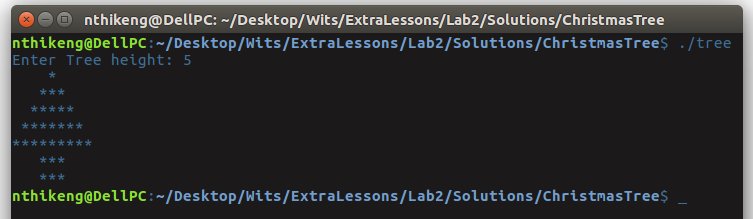
\includegraphics[width=0.8\columnwidth]{Tree} % Example image
	
	\textit{Figure 1: Christmas Tree}
\end{center}

% Numbered question, with an optional title
\subsection{Creating an Information Board*}
If you go to the Wits Bus Stop, you will notice that there is an information board that tells us the various time for departing buses. We will try to recreate some basic functionality of the board..
\\\\
You are given a text that has \textit{information-board-letters} that are separated by a \# , you are required to take an upper case word as input and print it to the terminal using the alphabets that are found in the text file.
\\\\
The figure below show the expected input and output
\begin{center}
	\includegraphics[width=0.8\columnwidth]{Hello} % Example image
	
	\textit{Figure 2: Information board}
\end{center}

\begin{warn} % Information block
This question is not for the feint hearted
\end{warn}

%----------------------------------------------------------------------------------------
%	PROBLEM 2
%----------------------------------------------------------------------------------------
\newpage
\section{Sieve of Eratosthenes}
This is an ancient alogorthim developed by Eratosthenes to find prime numbers. It works by finding the lowest prime number then discarding all the multiples of that prime. It will do so iteratively until there are no prime numbers left in the list.
\\\\
The sieve of Eratosthenes stops when the square of the number we are testing is greater than the last number on the grid (in our case 100).
\\\\
Since $11^2  = 121$ and $121>100$, when we get to the number 11, we can stop looking.

\begin{center}
	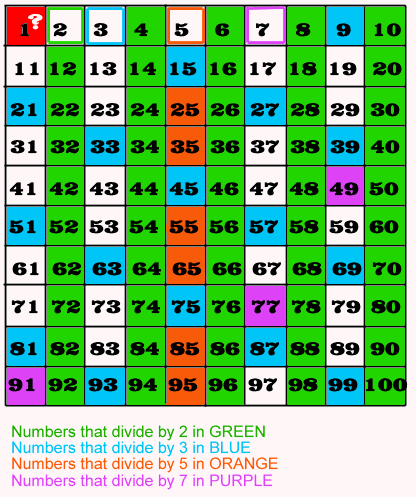
\includegraphics[width=0.5\columnwidth]{Sieve} % Example image	
	
	\textit{Figure 3: Sieve of Eratosthenes}
\end{center}
%----------------------------------------------------------------------------------------

\end{document}
